\section*{Introduction}
\addcontentsline{toc}{section}{Introduction}

Requirements analysis and specification is a crucial phase in the information system
development process. It consists, first and foremost, of clarifying the functional
and non-functional requirements of the system. This step then allows a complete
understanding of the subject in order to position oneself clearly, precisely and
without ambiguity.

% ── 2.1 ─────────────────────────────────────────────────────────────────────
\section{Requirements Analysis}

This step allows us to understand the overall context of our project, that is to say
to identify the main features and determine the actors who will interact with the
system.

\subsection{Identification of Actors}

Actors are entities external to the system (people, hardware, systems) that are
likely to exchange information with it. The following is a list of the actors who
will interact with our system:

\begin{longtable}{@{}P{0.21\linewidth}P{0.75\linewidth}@{}}
	\caption{List of MES application users}
	\label{tab:mescha-acteurs} \\
	\toprule
	\textbf{Actor} & \textbf{Description} \\
	\midrule
	\endfirsthead

	\toprule
	\textbf{Actor} & \textbf{Description} \\
	\midrule
	\endhead

	\multicolumn{2}{r}{\small Continued on next page} \\
	\endfoot

	\endlastfoot

	Administrator  &
	This is the person responsible for the MES platform. They manage all users
	(supervisors, operators), passwords and account statuses. They have access to all
	administration application dashboards. \\[6pt]

	Supervisor     &
	This is an intermediate user. They can monitor the progress of production operations
	on their work centre, view machine status and track the progress of production
	orders. Mark operation as finished or cancel/interupt uneeded operations. 
	View machine dashboards. Have access to all the access of the operators \\[6pt]

	Operator       &
	This is the end user of the MES application. Assigned to a work centre
	(\textit{Work Center}), they can view the production orders assigned to their machine,
	start, pause or resume an operation, declare produced quantities, declare defective 
	material, and scan components for consumption. \\

\end{longtable}

\subsection{Identification of Requirements}

At this stage, we will define the specific requirements of our
application, clearly distinguishing functional requirements from non-functional
requirements.

\subsubsection{Functional Requirements}

Each actor of the platform has specific expectations referred to as functional
requirements. To define the functional scope, it is necessary that the conceptual
solution meets these functional requirements.

\begin{itemize}
	\item \textbf{Authentication}: This feature allows any user to log in to the
	      platform using their Auth~ID and password. Upon first login, the user is prompted
	      to change their temporary password. A secure session token (GUID, 12~h validity) is
	      issued upon each successful login.

	\item \textbf{Two-Factor Authentication (2FA)}: When enabled globally by the
	      administrator, users must complete a second authentication step by scanning their
	      personal badge QR~code after entering their credentials. Administrators can view,
	      print, and regenerate badge secrets for any user.

	\item \textbf{Application Setup}: On first launch, the user must configure the
	      middleware host URL (entered manually or obtained by scanning a QR~code) so that
	      the application connects to the correct server instance. The host is persisted
	      across sessions and can be changed from the login page.

	\item \textbf{User Management}: This feature allows the administrator to:
	      \begin{itemize}
	      	\item View the complete list of MES users.
	      	\item Create a new user account by linking it to a Business
	      	      Central employee and assigning them a role and work centre(s) if needed.
	      	\item Generate and assign a temporary password.
	      	\item Activate or deactivate an account (automatic revocation of active tokens).
	      	\item Change a user's role (Operator, Supervisor, Administrator) and work centre assignment.
	      	\item View, print, and regenerate a user's badge QR~code for 2FA purposes.
	      \end{itemize}

	\item \textbf{Security Policy}: The administrator can configure a password rotation
	      period (in days). A scheduled background job runs every 24~hours and flags users
	      whose password age exceeds the configured period, forcing them to change their
	      password on next login.

	\item \textbf{Machine Management}: This feature allows users to:
	      \begin{itemize}
	      	\item View the list of machines in a work centre with their current status
	      	       (Idle, Working).
	      	\item View the production order currently running on each machine.
	      \end{itemize}

	\item \textbf{Production Order Management}: This feature allows the \userrole{Operator} and the \userrole{supervisor} to:
	      \begin{itemize}
	      	\item View production orders (Planned, Firm, Released) assigned to their machine.
	      	\item Filter and sort orders by status or date.
	      	\item View the details of an order (item, quantity, planned dates, operation
	      	      description).
	      \end{itemize}

	\item \textbf{Production Operation Management}: This feature is the core of the
	      system. It allows the operator or Supervisor to:
	      \begin{itemize}
	      	\item Start an operation (validation of prerequisites: released order, free machine, previous operation completed if applicable).
	      	\item Pause or resume an ongoing operation.
		 	\item Declare produced quantities (validation: quantity $> 0$, no excess of the ordered quantity).
	      	\item View progress in real time (produced quantity, completion percentage, operation status, scrapped units).
			\item View the Bill of Materials for the current operation with component consumption
	      	\item Report scrapped units with a reason code.
	      	\item scan components into the operation to record consumption against the BOM.
	      \end{itemize}

	\item \textbf{Progress Dashboard}: Allows the operator and supervisor to view all
	      active operations (Running / Paused) on a given machine, with their respective
	      progress.

	\item \textbf{Password Change}: Allows any logged-in user to change their password
	      by entering their old password and the new one.

	\item \textbf{AI Chat Assistant}: An embedded natural-language assistant allows
	      operators and supervisors to query machine status, production progress, scrap
	      data, BOM, and history without navigating the full interface. The assistant
	      resolves ambiguous machine references, answers fleet-wide questions, surfaces
	      operational anomalies, and provides contextual navigation shortcuts.
\end{itemize}

\subsubsection{Non-Functional Requirements}

To define the non-functional scope, it is necessary that the conceptual solution meets
these non-functional requirements:

\begin{itemize}
	\item \textbf{Performance}: The platform performs efficiently in terms of handling
	      routine operations (login, order consultation, production declaration).

	\item \textbf{Security}: Implementation of a token-based authentication system
	      (signed GUID, 12~h expiry) and role management (Admin, Supervisor, Operator) to
	      control access to features. Passwords are stored as SHA-256 hashes with a salt.
	      Optional two-factor authentication enforces badge QR verification as a second
	      factor. A configurable password expiry policy forces periodic credential rotation.

	\item \textbf{Maintainability}: The AL back-end code is organised in layers
	      (Tables, Enums, Codeunits, API Pages) and the Flutter code follows a layered
	      architecture (Data, Domain, Presentation) with the Provider pattern, facilitating
	      updates and the addition of new features.

	\item \textbf{Ergonomics}: The user interface is adaptive (mobile, tablet, PC)
	      thanks to responsive layouts dedicated to each form factor, minimising the learning
	      curve for workshop operators.

	\item \textbf{Portability}: The Flutter application is compiled for Android, iOS,
	      Web, Linux, macOS and Windows from a single codebase. The Business Central back-end
	      is deployable both on-premises and in SaaS (cloud) mode.
\end{itemize}

% ── 2.2 ─────────────────────────────────────────────────────────────────────
\section{Project Management with Scrum}

\subsection{Backlog Features}

% ===================== DOMAIN 1: AUTHENTICATION & USER MANAGEMENT =====================
\subsubsection{Domain 1: Authentication \& User Management}
\label{domain1}

\vspace{0.3cm}

\begin{longtable}{p{1.5cm} p{5cm} p{6.5cm} p{2cm}}
	\hline
	\textbf{ID} & \textbf{User Story} & \textbf{Acceptance Criteria} & \textbf{Priority} \\
	\hline
	\endfirsthead

	\hline
	\textbf{ID} & \textbf{User Story} & \textbf{Acceptance Criteria} & \textbf{Priority} \\
	\hline
	\endhead

	\multicolumn{4}{r}{\small Continued on next page} \\
	\endfoot

	\endlastfoot

	\textbf{US-1.1} &
	As an \userrole{Administrator}, I need to assign a user account for each employee  so
	that users only access features appropriate to their role.
	& \begin{itemize}[noitemsep, topsep=0pt, partopsep=0pt, leftmargin=*]
	\item Ability to assign a user as \userrole{Operator} or \userrole{Supervisor} or \userrole{Administrator}.
	\item Unauthorized actions are blocked with clear error messages.
	\end{itemize} &
	High \\
	\midrule

	\textbf{US-1.2} &
	As a User (\userrole{Operator} / \userrole{Supervisor} / \userrole{Administrator}),
	I need to log into the system with my credentials so that I can access
	features appropriate to my role.
	&
	\begin{itemize}[noitemsep, topsep=0pt, partopsep=0pt, leftmargin=*]
	\item User can enter username and password.
	\item System validates credentials against the \techname{MES}.
	\item Session token is created upon successful authentication.
	\item User is redirected to the appropriate dashboard based on role.
	\end{itemize} &
	High \\
	\midrule

	\textbf{US-1.3} &
	As an \userrole{Administrator}, I need to search users.
	& \begin{itemize}[noitemsep, topsep=0pt, partopsep=0pt, leftmargin=*]
	\item Ability to filter users based on their role.
	\item Ability to search for a specific user.
	\end{itemize} &
	High \\
	\midrule

	\textbf{US-1.4} &
	As an \userrole{Administrator}, I need to see a list of all
	users with their details so that I can manage their accounts.
	& \begin{itemize}[noitemsep, topsep=0pt, partopsep=0pt, leftmargin=*]
	\item The user list displays each account's full name, email, role, when he was active, and work centre.
	\item Clicking on the action button shows a dropdown menu with available actions(change role, generate password, view badge, and toggle activation).
	\item The list refreshes automatically after a new user is created.
	\end{itemize} & High \\ \midrule

	\textbf{US-1.5} &
	As an \userrole{Administrator}, I need to generate and assign temporary
	passwords to users so that they can log in for the first time.
	& \begin{itemize}[noitemsep, topsep=0pt, partopsep=0pt, leftmargin=*]
	\item Admin can generate a random secure password for any user.
	\item The generated password is sent to the \techname{ERP} via \texttt{AdminSetPassword}.
	\item The target account is flagged \domainterm{Need To Change Password} after the password is set.
	\item Success or failure is reported to the admin with a clear message.
	\end{itemize} & High \\ \midrule

	\textbf{US-1.6} &
	As an \userrole{Administrator}, I need to change the role and work-centre
	assignment of an existing user so that access rights stay current.
	&
	\begin{itemize}[noitemsep, topsep=0pt, partopsep=0pt, leftmargin=*]
	\item Admin can select a new role for any other user.
	\item Work-centre list updates based on the selected role.
	\item All active tokens for the target user are revoked on save.
	\item The user list refreshes after a successful change.
	\end{itemize}
	&
	High \\ \midrule

	\textbf{US-1.7} &
	As an \userrole{Administrator}, I need to activate or deactivate a user
	account so that access can be revoked without deleting the account.
	&
	\begin{itemize}[noitemsep, topsep=0pt, partopsep=0pt, leftmargin=*]
	\item Admin can toggle the active status of any other user.
	\item Deactivation immediately revokes all active tokens.
	\item The user row updates its visual status indicator immediately.
	\end{itemize}
	&
	High \\ \midrule

	\textbf{US-1.8} &
	As a User (\userrole{Operator} / \userrole{Supervisor} / \userrole{Administrator}),
	I need to complete a badge QR code scan after entering my credentials so
	that my identity is verified by a second factor.
	&
	\begin{itemize}[noitemsep, topsep=0pt, partopsep=0pt, leftmargin=*]
	\item \domainterm{2FA} prompt appears only when \domainterm{TwoFA Enabled} is active in \techname{MES Settings}.
	\item Camera opens and scans a QR badge code.
	\item Manual entry field available as a fallback.
	\item Session token is persisted only after successful badge verification.
	\item Failed scan shows an error; scanner reactivates.
	\item User can cancel and return to the login page.
	\end{itemize}
	&
	High \\ \midrule

	\textbf{US-1.9} &
	As an \userrole{Administrator}, I need to view, print, and regenerate a
	user's badge QR~code so that I can distribute it and invalidate a lost or
	compromised badge.
	&
	\begin{itemize}[noitemsep, topsep=0pt, partopsep=0pt, leftmargin=*]
	\item Badge QR rendered from the user's \domainterm{Badge Secret} via a barcode widget.
	\item Print button generates a PDF.
	\item Regenerate action shows a confirmation dialog before replacing the secret.
	\item New QR is displayed immediately after regeneration.
	\end{itemize}
	&
	High \\ \midrule

	\textbf{US-1.10} &
	As an \userrole{Administrator}, I need to globally enable or disable \domainterm{2FA}
	and configure a password rotation period so that I can control the
	organisation's authentication security level.
	&
	\begin{itemize}[noitemsep, topsep=0pt, partopsep=0pt, leftmargin=*]
	\item \domainterm{2FA} toggle and password rotation period field available on a \uilabel{Settings} page.
	\item Changes take effect on the next login attempt.
	\item Settings are persisted.
	\item A scheduled job (every 24~h) flags users whose password age exceeds the configured period.
	\item Unsaved changes display a persistent banner with \uilabel{Discard} and \uilabel{Save} actions.
	\end{itemize}
	&
	High \\ \midrule

	\textbf{US-1.11} &
	As a first-time user, I need to configure the middleware host URL (or scan
	a QR~code) so that the application connects to the correct server instance.
	&
	\begin{itemize}[noitemsep, topsep=0pt, partopsep=0pt, leftmargin=*]
	\item \uilabel{Paring} page shown on first launch when no host is saved.
	\item URL can be entered manually or obtained by scanning a QR~code.
	\item URL is validated (no spaces, no illegal characters).
	\item Saved host persists across app restarts.
	\item \uilabel{Change Host} link on the login page allows re-entering the pairing screen.
	\end{itemize}
	&
	High \\
	\midrule

	\textbf{US-1.12} &
	As an \userrole{Administrator}, I need to export the list of users so that
	I can use the information in other applications or processes.
	& \begin{itemize}[noitemsep, topsep=0pt, partopsep=0pt, leftmargin=*]
	\item The ability to export all user info.
	\item The information is structured in the form of an excel file.
	\end{itemize} &
	Medium \\
	\bottomrule
\end{longtable}


% ===================== DOMAIN 2: MACHINE MONITORING =====================
\subsubsection{Domain 2: Machine \& Production Management}
\label{domain2}

\vspace{0.3cm}

\begin{longtable}{ p{1.5cm} p{5cm} p{6.5cm} p{2cm} }
	\toprule
	\textbf{ID} & \textbf{User Story} & \textbf{Acceptance Criteria} & \textbf{Priority} \\
	\midrule
	\endfirsthead

	\toprule
	\textbf{ID} & \textbf{User Story} & \textbf{Acceptance Criteria} & \textbf{Priority} \\
	\midrule
	\endhead

	\multicolumn{4}{r}{\small Continued on next page} \\
	\endfoot

	\endlastfoot

	\textbf{US-2.1} &
	As an \userrole{Operator} or \userrole{Supervisor}, I need to see the list
	of machines in my work center with their current status so that I can see
	which machines are currently active.
	& \begin{itemize}[noitemsep, topsep=0pt, partopsep=0pt, leftmargin=*]
	\item Machine list is scoped to the authenticated user's work centre.
	\item Each card shows machine name, current status (\domainterm{Idle},
	\domainterm{Working}), active production order number, operation No, item No, and
	the item name.
	\item The list refreshes automatically every 20 seconds.
	\end{itemize} &
	High \\
	\midrule

	\textbf{US-2.2} &
	As an \userrole{Operator} or \userrole{Supervisor}, I need to view the operations of the
	production orders assigned to a machine so that I know what work needs
	to be done.
	& \begin{itemize}[noitemsep, topsep=0pt, partopsep=0pt, leftmargin=*]
	\item Only \domainterm{Planned}, \domainterm{Firm Planned}, or
	\domainterm{Released} orders are shown.
	\item Each card displays order number, item description, planned quantity,
	planned start and end dates, operation description, and operation number.
	\end{itemize} &
	High \\
	\midrule

	\textbf{US-2.3} &
	As an \userrole{Operator} or \userrole{Supervisor}, I need to start a
	production operation so that the system records that the order has begun.
	& \begin{itemize}[noitemsep, topsep=0pt, partopsep=0pt, leftmargin=*]
	\item Only \domainterm{operation} from \domainterm{Released} orders may be started.
	\item An operation cannot be started if it is already running.
	\item A machine cannot run two operations simultaneously.
	\item A new MES Operation State record is created with status change so it can be tracked.
	\item The previous operation in the same production order (if any) must be
	\domainterm{Finished}, \domainterm{Interrupted}, or currently \domainterm{Running}
	with enough send-ahead quantity.
	\end{itemize} & High \\ \midrule

	\textbf{US-2.4} &
	As a \userrole{Supervisor} or \userrole{Operator}, I need to monitor the
	current status of all active operations on a machine so that I can follow
	the progress of each order.
	& \begin{itemize}[noitemsep, topsep=0pt, partopsep=0pt, leftmargin=*]
	\item The Operations Progress tab shows all operations whose latest status
	record is \domainterm{Running} or \domainterm{Paused}.
	\item Each card shows order number, operation number, current status, operation description,
	last updated timestamp, and progress.
	\item Data refreshes automatically every 5 seconds.
	\end{itemize} & High \\ \midrule

	\textbf{US-2.5} &
	As an \userrole{Operator} or \userrole{Supervisor}, I need a tabbed view
	for a machine so that I can navigate between pending orders and active
	operation progress without leaving the machine context.
	& \begin{itemize}[noitemsep, topsep=0pt, partopsep=0pt, leftmargin=*]
	\item Selecting a machine from the list opens a dedicated machine page.
	\item The page provides three tabs: \domainterm{Orders},
	\domainterm{Progress}, and \domainterm{History}.
	\item The active tab is visually highlighted in the navigation bar.
	\end{itemize} & High \\ \midrule

	\textbf{US-2.6} &
	As an \userrole{Operator} or \userrole{Supervisor}, I need to filter and
	sort production orders so that I can quickly find the most relevant work.
	& \begin{itemize}[noitemsep, topsep=0pt, partopsep=0pt, leftmargin=*]
	\item Orders can be searched by order number, item description, or date.
	\item Orders can be filtered by status (\domainterm{All}, \domainterm{Planned},
	\domainterm{Firm Planned}, \domainterm{Released}).
	\item Orders can be sorted by planned start date ascending or descending.
	\item On mobile, the status filter is accessible via a compact popup menu.
	\end{itemize} & High \\ \midrule

	\textbf{US-2.7} &
	As a \userrole{Supervisor} or \userrole{Operator}, I need to view the
	history of completed operations for a machine so that I can audit past
	production.
	&
	\begin{itemize}[noitemsep, topsep=0pt, partopsep=0pt, leftmargin=*]
	\item The History tab shows all operations with status
	\domainterm{Finished},\domainterm{Interrupted}, or \domainterm{Cancelled}.
	\item Each card shows order number, status, product name, produced
	quantity, start time, and end time.
	\item The list supports free-text search and sort by start date.
	\item Tapping a card navigates to the full operation detail page.
	\end{itemize}
	&
	High \\
	\bottomrule
\end{longtable}


\subsubsection{Domain 3: Production Execution \& Traceability}
\label{domain3}

\vspace{0.3cm}

\begin{longtable}{p{1.5cm} p{5cm} p{6.5cm} p{2cm}}
	\hline
	\textbf{ID} & \textbf{User Story} & \textbf{Acceptance Criteria} & \textbf{Priority} \\
	\hline
	\endfirsthead
	\hline
	\textbf{ID} & \textbf{User Story} & \textbf{Acceptance Criteria} & \textbf{Priority} \\
	\hline
	\endhead
	\multicolumn{4}{r}{\small Continued on next page} \\
	\endfoot
	\endlastfoot

	\textbf{US-3.1} &
	As an \userrole{Operator} or \userrole{Supervisor}, I need to declare the
	quantity produced in a cycle so that the system records production progress.
	&
	\begin{itemize}[noitemsep, topsep=0pt, partopsep=0pt, leftmargin=*]
	\item Declared quantity must be positive and not exceed remaining quantity that need to be produced.
	\item Declared quantity must be less than the amount that can be produced with the available components scanned remaining.
	\item Each declaration creates a new progression cycle record.
	\item Produced quantity and progress percentage update immediately.
	\end{itemize}
	& High \\ \midrule

	\textbf{US-3.2} &
	As an \userrole{Operator} or \userrole{Supervisor}, I need to pause and
	resume an active operation so that interruptions are tracked accurately.
	&
	\begin{itemize}[noitemsep, topsep=0pt, partopsep=0pt, leftmargin=*]
	\item A Running operation can be paused; a Paused one can be resumed.
	\item A machine cannot resume if another operation is already running.
	\end{itemize}
	& High \\ \midrule

	\textbf{US-3.3} &
	As a \userrole{Supervisor}, I need to finish, interrupt or cancel an operation so that
	the machine is released and the order is closed in the system.
	&
	\begin{itemize}[noitemsep, topsep=0pt, partopsep=0pt, leftmargin=*]
	\item Finishing a complete order (100\%) shows a green confirmation dialog.
	\item Interrupting or Cancelling an operation shows a red warning dialog.
	\item If the operation is started then it is marked as interrupted otherwise as cancelled
	\item Closing sets the execution end time and inserts an Idle machine status.
	\end{itemize}
	& High \\ \midrule

	\textbf{US-3.4} &
	As an \userrole{Operator} or \userrole{Supervisor}, I need a dedicated
	operation detail page with up-to-date data in one place.
	&
	\begin{itemize}[noitemsep, topsep=0pt, partopsep=0pt, leftmargin=*]
	\item Shows status, order number, product, required and produced quantities.
	\item The information updates automatically without a manual refresh.
	\end{itemize}
	& High \\ \midrule

	\textbf{US-3.5} &
	As an \userrole{Operator} or \userrole{Supervisor}, I need to see all
	production cycles declared for an operation.
	&
	\begin{itemize}[noitemsep, topsep=0pt, partopsep=0pt, leftmargin=*]
	\item Cycle table lists operator, quantity, cumulative total, and timestamp.
	\item Records ordered newest-first with pagination.
	\item Updates after each new declaration.
	\end{itemize}
	& High \\ \midrule

	\textbf{US-3.6} &
	As an \userrole{Operator} or \userrole{Supervisor}, I need a visual chart
	of declarations over time to identify performance trends.
	&
	\begin{itemize}[noitemsep, topsep=0pt, partopsep=0pt, leftmargin=*]
	\item Line chart plots cycle quantity vs.\ declaration time.
	\item Touch tooltip shows operator, quantity, total production, timestamp.
	\item Auto-scrolls to most recent data point on load and refresh.
	\end{itemize}
	& Medium \\ \midrule

	\textbf{US-3.7} &
	As an \userrole{Operator} or \userrole{Supervisor}, I need to see the Bill
	of Materials for an operation to know which components are required.
	&
	\begin{itemize}[noitemsep, topsep=0pt, partopsep=0pt, leftmargin=*]
	\item Components are colour-coded by remaining amount (the needed amount (green) / less then necessary to make a single item (red) otherwise (yellow)).
	\item BOM data refreshes after every consumption event.
	\item can be expanded to a dialog for a better view on larger screens.
	\item search by name and filter by state
	\end{itemize}
	& High \\ \midrule

	\textbf{US-3.8} &
	As an \userrole{Operator} or \userrole{Supervisor}, I need to report
	scrapped units with a reason code so that waste is accurately tracked.
	&
	\begin{itemize}[noitemsep, topsep=0pt, partopsep=0pt, leftmargin=*]
	\item Scrap can only be declared when the operation is Running.
	\item A reason code must be selected before submission.
	\item Need to select either input material or output scrap.
	\item the quantity of scrapped units cannot exceed the quantity 
	that can be produced with the available components scanned remaining.
	\item Each declaration's quantity, code, and operator is stored for tracibility.
	\end{itemize}
	& High \\ \midrule

	\textbf{US-3.9} &
	As a \userrole{Supervisor}, I need to declare production or scrap on behalf of an
	operator so that output is attributed to the correct person.
	&
	\begin{itemize}[noitemsep, topsep=0pt, partopsep=0pt, leftmargin=*]
	\item Supervisor role sees an operator selector in the declare dialog.
	\item Selected operator's ID is stored with the declaration record for tracibility.
	\item If no operator is selected, it is declared as if the supervisor made the declaration.
	\end{itemize}
	& Medium \\ \midrule

	\textbf{US-3.10} &
	As an \userrole{Operator} or \userrole{Supervisor}, I need to scan
	components into an operation so that consumption is recorded against the BOM.
	&
	\begin{itemize}[noitemsep, topsep=0pt, partopsep=0pt, leftmargin=*]
	\item any camera connected to the device reads  barcodes.
	\item Duplicate scan increments quantity on the existing row.
	\item Confirming scans inserts consumption records and refreshes the BOM.
	\item After confirmation, the inventory in the ERP is updated to reflect the consumed quantity.
	\end{itemize}
	& High \\ \midrule

	\textbf{US-3.11} &
	As an \userrole{Operator} or \userrole{Supervisor}, I need to print a label
	for a production order so that produced parts are correctly identified.
	&
	\begin{itemize}[noitemsep, topsep=0pt, partopsep=0pt, leftmargin=*]
	\item Label includes DataMatrix barcode encoding order, machine, item data.
	\item PDF generation supports landscape/portrait toggle.
	\item Print button available only when operation is Finished or progress
	$\geq$ 100\%.
	\end{itemize}
	& Medium \\ \midrule

	\textbf{US-3.12} &
	As an \userrole{Operator} or \userrole{Supervisor}, I need a label printed
	for each declared unit so that individual pieces carry traceable information.
	&
	\begin{itemize}[noitemsep, topsep=0pt, partopsep=0pt, leftmargin=*]
	\item One PDF page per declared unit with a label counter.
	\item Same DataMatrix encoding as the production label.
	\item Launched automatically after a successful production declaration.
	\end{itemize}
	& Medium \\
	\bottomrule
\end{longtable}


% ===================== DOMAIN 4: ADMINISTRATION =====================
\subsubsection{Domain 4: Administration \& Monitoring}
\label{domain4}

\vspace{0.3cm}

\begin{longtable}{p{1.5cm} p{5cm} p{6.5cm} p{2cm}}
	\hline
	\textbf{ID} & \textbf{User Story} & \textbf{Acceptance Criteria} & \textbf{Priority} \\
	\hline
	\endfirsthead
	\hline
	\textbf{ID} & \textbf{User Story} & \textbf{Acceptance Criteria} & \textbf{Priority} \\
	\hline
	\endhead
	\multicolumn{4}{r}{\small Continued on next page} \\
	\endfoot
	\endlastfoot

	\textbf{US-4.1} &
	As an \userrole{Supervisor}, I need a performance dashboard for all
	machines so that I can monitor production health across the facility.
	&
	\begin{itemize}[noitemsep, topsep=0pt, partopsep=0pt, leftmargin=*]
	\item Dashboard shows uptime, operation cancelled or finished count, total produced, and scrap
	per machine.
	\item Configurable time-range (hours back) filter.
	\end{itemize}
	& High \\ \midrule

	\textbf{US-4.2} &
	As an \userrole{Administrator}, I need a filterable activity log
	of all system actions so that I can audit operator and machine activity.
	&
	\begin{itemize}[noitemsep, topsep=0pt, partopsep=0pt, leftmargin=*]
	\item Log entries includes all the relevant fields with timestamps.
	\item Filterable by action type and time range.
	\end{itemize}
	& High \\ \midrule


	\textbf{US-4.3} &
	As any user, I need the application available in English, French, and Arabic
	so that I can use it in my preferred language.
	&
	\begin{itemize}[noitemsep, topsep=0pt, partopsep=0pt, leftmargin=*]
	\item Language selector on login screen and in profile page.
	\item All UI strings externalised; no hard-coded text.
	\item Arabic locale activates RTL layout automatically.
	\item Language preference persisted across sessions in the same device.
	\end{itemize}
	& High \\ \midrule

	\textbf{US-4.4} &
	As a first-time user, I need guided coach-mark tutorials so that I can learn
	the interface without external documentation.
	&
	\begin{itemize}[noitemsep, topsep=0pt, partopsep=0pt, leftmargin=*]
	\item Tutorials shown exactly once per install per screen.
	\item Coach marks cover: machine list, machine detail tabs, operation
	detail, and admin dashboard.
	\item Localised skip button text.
	\end{itemize}
	& Medium \\
	\bottomrule
\end{longtable}


% ===================== DOMAIN 5: AI ASSISTANT =====================
\subsubsection{Domain 5: AI Chat Assistant \& Analytical Intelligence}
\label{domain5}

\vspace{0.3cm}

\begin{longtable}{p{1.5cm} p{5cm} p{6.5cm} p{2cm}}
	\hline
	\textbf{ID} & \textbf{User Story} & \textbf{Acceptance Criteria} & \textbf{Priority} \\
	\hline
	\endfirsthead
	\hline
	\textbf{ID} & \textbf{User Story} & \textbf{Acceptance Criteria} & \textbf{Priority} \\
	\hline
	\endhead
	\multicolumn{4}{r}{\small Continued on next page} \\
	\endfoot
	\endlastfoot

	\textbf{US-5.1} &
	As an \userrole{Operator} or \userrole{Supervisor}, I need a natural-language
	chat assistant so that I can query machine status, production progress, and
	operational data without navigating the full UI.
	&
	\begin{itemize}[noitemsep, topsep=0pt, partopsep=0pt, leftmargin=*]
	\item Chat panel opens as a side overlay on wide screens and as a dialog on mobile.
	\item Assistant answers questions about machines, orders, live operations, BOM,
	history, and scrap.
	\item Responses are scoped to the user's own work centres (access control enforced).
	\item Multi-turn conversation history is maintained within the session.
	\item Conversation can be cleared by the user.
	\end{itemize}
	& High \\ \midrule

	\textbf{US-5.2} &
	As an \userrole{Operator} or \userrole{Supervisor}, I need the assistant to
	resolve ambiguous machine references (e.g.\ ``Fraiseuse~3'') so that I do not
	need to know exact machine codes.
	&
	\begin{itemize}[noitemsep, topsep=0pt, partopsep=0pt, leftmargin=*]
	\item Machine names, partial codes, and digit-only references are matched to
	the correct machine using a five-tier fuzzy resolution strategy.
	\item High-confidence matches ($\geq$ 85\%) are resolved silently.
	\item Low-confidence matches present up to 3 candidates for disambiguation.
	\item Machine access control is enforced after resolution.
	\end{itemize}
	& High \\ \midrule

	\textbf{US-5.3} &
	As an \userrole{Operator} or \userrole{Supervisor}, I need the assistant to
	answer fleet-wide questions (e.g.\ ``which machines are running?'') so that I
	get a consolidated view without visiting each machine individually.
	&
	\begin{itemize}[noitemsep, topsep=0pt, partopsep=0pt, leftmargin=*]
	\item Queries about all machines trigger a parallel fan-out across work centres.
	\item Results are filtered by running / idle / overdue / scrap status as requested.
	\item Fan-out is capped to control response time.
	\item Fleet summary includes machine count, utilisation percentage, and active orders.
	\end{itemize}
	& High \\ \midrule

	\textbf{US-5.4} &
	As an \userrole{Operator} or \userrole{Supervisor}, I need the assistant to
	provide contextual navigation shortcuts so that I can open a machine, operation,
	or dashboard directly from the chat response.
	&
	\begin{itemize}[noitemsep, topsep=0pt, partopsep=0pt, leftmargin=*]
	\item Chat responses include up to 4 action buttons when a redirect is relevant.
	\item Tapping an action navigates to the corresponding screen.
	\item Action buttons appear only on the last assistant message.
	\end{itemize}
	& Medium \\ \midrule

	\textbf{US-5.5} &
	As a \userrole{Supervisor}, I need the assistant to proactively highlight
	anomalies (overdue orders, scrap spikes, idle operators) so that I can act
	before problems escalate.
	&
	\begin{itemize}[noitemsep, topsep=0pt, partopsep=0pt, leftmargin=*]
	\item Scrap rate above 5\% is flagged as a warning; above 15\% as critical.
	\item Scrap spikes (recent rate $>$ 2.5$\times$ baseline) are explicitly mentioned.
	\item Overdue orders (past planned end) and at-risk orders ($<$ 4~h remaining)
	are highlighted.
	\item Paused operations exceeding the configured threshold are surfaced.
	\end{itemize}
	& High \\
	\bottomrule
\end{longtable}

% ── 2.3 ─────────────────────────────────────────────────────────────────────

\section{Sprint Plan}

The project was organised into five two-week sprints, each delivering a
functional increment verified by a sprint review with the professional supervisor.

\begin{longtable}{@{} P{0.10\linewidth} P{0.30\linewidth} P{0.55\linewidth} @{}}
	\caption{MES project sprint plan}
	\label{tab:mescha-sprint_plan} \\
	\toprule
	\textbf{Sprint} & \textbf{Domain}                                   & \textbf{Scope} \\
	\midrule
	\endfirsthead

	\toprule
	\textbf{Sprint} & \textbf{Domain}                                   & \textbf{Scope} \\
	\midrule
	\endhead

	\multicolumn{3}{r}{\small Continued on next page} \\
	\endfoot

	\endlastfoot

	Sprint~1        & Authentication \& User Management                 &
	Secure login,2 factor authentification(2FA), change password, profile page
	and session token management, role-based access control, administrator user
	creation, password generation and reset, role and work-centre change, account
	activation/deactivation, badge management (view, print, regenerate), password
	expiry	policy configuration, export users and first-launch host pairing. \\ \midrule

	Sprint~2        & Machine Monitoring \& Production Order Management &
	Real-time machine status tracking, production order list per machine,
	operation start, tabbed machine view with Orders / Progress / History tabs,
	order filtering and sorting. \\ \midrule

	Sprint~3        & Production Execution \& Traceability              &
	Production cycle declarations, pause/resume/finish/cancel/interupt operations,
	operation detail page with up-to-date data, production chart, Bill of Materials
	visibility, component barcode scanning, scrap declaration,
	supervisor proxy declaration, and label printing. \\ \midrule

	Sprint~4        & Administration and System Monitoring \& Configuration              &
	Monitoring dashboard and Administrator activity log, barcode view and printing, user
	export, multi-language support (EN/FR/AR) and RTL layout, in-app onboarding tutorials. \\ \midrule

	Sprint~5        & AI Assistant \& Analytical Intelligence           &
	Natural-language chat assistant, \techname{Node.js} reverse proxy middleware,
	\techname{Python} AI agent with intent classification, multi-provider LLM support,
	fuzzy machine resolution, composite fan-out queries, data enrichment,
	anomaly detection (scrap spikes, overdue orders), and contextual
	redirect actions. \\
	\midrule
\end{longtable}

\section{Global Application Architecture}

\subsection{Physical Architecture}

The physical architecture of the MES system rests on three main nodes:

	\begin{itemize}
	    \item \textbf{Business Central Server (on-premises / SaaS)}: hosts the AL extension
	    that exposes OData V4 endpoints and the business REST APIs. In on-premises mode, the
	    server runs on a BC210 instance accessible on port 7048. In SaaS mode, the base URLs
	    follow the schema
	    \texttt{api.businesscentral.dynamics.com/v2.0/<tenantId>/<environment>/ODataV4/}.

	    \item \textbf{Node.js Middleware}: a reverse-proxy layer running between the Flutter
	    client and Business Central. It handles SSPI/Windows authentication toward BC,
	    exposes a unified REST API consumed by Flutter, and routes AI chat requests to the Python
	    AI agent.

	    \item \textbf{Flutter Client (mobile / web / desktop)}: application compiled for
	    Android, iOS, Web or desktop, communicating with the Node.js middleware via HTTP
	    requests. The middleware proxies these to the BC OData V4 endpoints.
		
		\item \textbf{A Python AI agent (Server)}: a module that acts as an interface between
		the application and the llm model chosen,includes intent classification tool calls.
	\end{itemize}

% IMAGE PLACEHOLDER - physical architecture diagram (BC server + Flutter clients)


\begin{figure}[H]
	\centering
	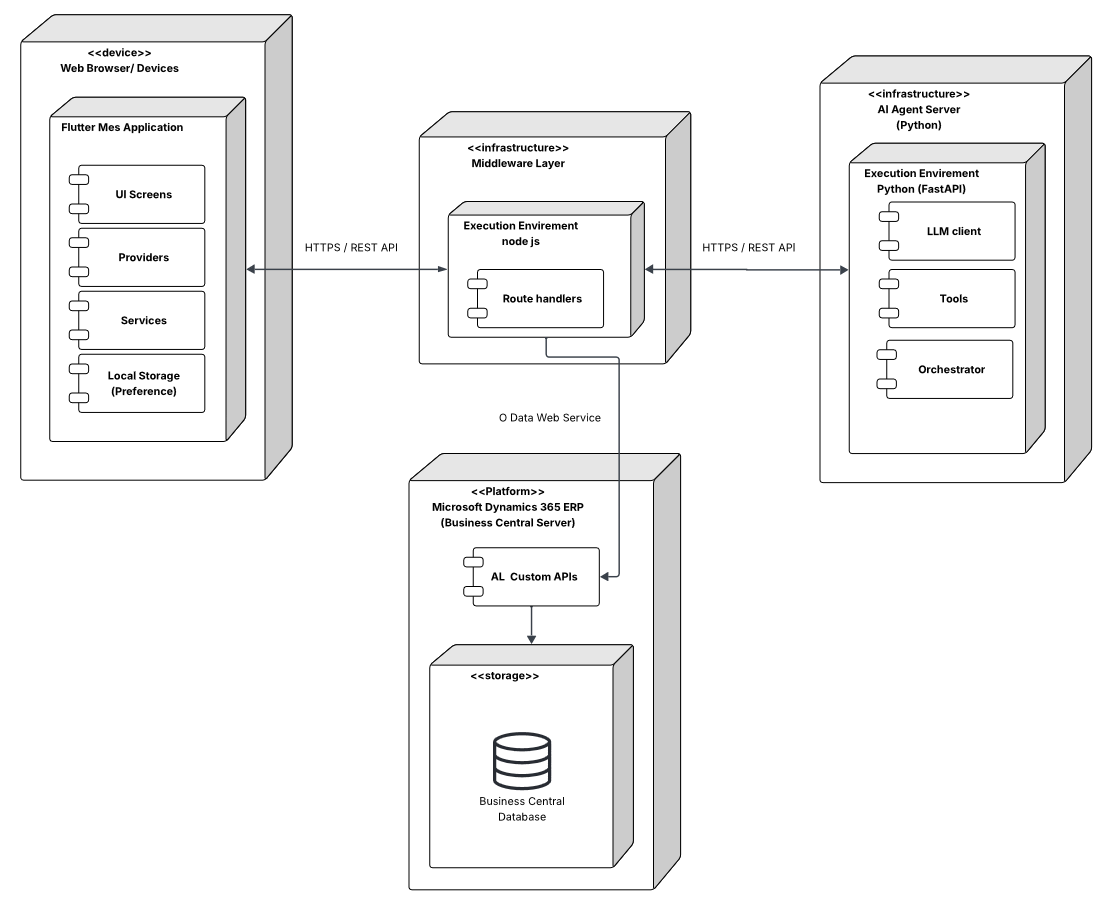
\includegraphics[width=\linewidth,keepaspectratio]{./media/MES_chapter-2-repport/systemArchitecture.png}
	\caption{MES System Physical Architecture}
	\label{fig:mescha-archi_physique}
\end{figure}

\subsection{Software Architecture}

The software architecture of the system is organised around four distinct layers.

\subsubsection{AL Back-end (Business Central)}

The back-end is structured in five layers:

\begin{itemize}
	\item \textbf{Tables (1-Tables)}: define the persistent data model; 
	MES User, MES Auth Token, MES Machine Status, MES Operation State, 
	MES Operation Scrap, MES Operation Execution, MES Operation Progression,
	MES Settings, MES Component Scan, and MES User Execution Interaction.
	\item \textbf{Enums (2-Enum)}: define the enumerated types; MES User 
	Role (Operator, Supervisor, Admin), MES Machine Status (Idle, Working), 
	MES Operation State (Running, Paused, Finished, Cancelled, Interrupted), 
	MES Token State (Revoked, Pending, Active).
	\item \textbf{Codeunits (3-CodeUnit)}: contain the business logic; 
	MES Auth Mgt (authentication, tokens), MES Password Mgt (SHA-256 hashing), 
	MES Machine Fetch (read operations), MES Machine Write (state orchestration),
	MES Machine Insert (table writes), MES Machine Validation (business rule guards),
	MES Authentification (user authentication), and the \domainterm{Mes Web Service}
	(wrappers exposed as web services).
	\item \textbf{API Pages (4-API)}: expose data for reading/writing via the BC REST 
	API; employees, work centres.
	\item \textbf{Pages (5-Pages)}: administration and debugging interfaces 
	in the BC client (lists, cards, API debug page, etc...).
\end{itemize}

\subsubsection{Node.js Middleware}

	The Node.js middleware is the network bridge between the Flutter client and
	Business Central. It handles SSPI/Windows authentication for BC OData V4
	requests, exposes a unified REST API to the Flutter application, and routes
	AI chat requests (\texttt{POST /api/ai/chat}) to the Python AI agent.

\subsubsection{Python AI Agent}

The Python AI agent (FastAPI) provides the conversational intelligence layer.
It classifies user intent, executes tool chains against Business Central via
the Node.js middleware, enriches results with data-analysis helpers, and
synthesises natural-language replies using a configurable multi-provider LLM client.


\subsubsection{Flutter Front-end}

The Flutter front-end follows a three-layer architecture:

\begin{itemize}
	\item \textbf{Data}: contains data models (models) and HTTP services (services) that
	      communicate with BC endpoints via the \texttt{http} library.
	\item \textbf{Domain}: contains the providers (Provider pattern) that expose the
	      application state to widgets --- AuthProvider, MesUserProvider,
	      MesMachinesProvider, MachineordersProvider, etc.
	\item \textbf{Presentation}: contains the pages and widgets of the user interface,
	      organised by functional domain (auth, admin, machine) with dedicated responsive
	      layouts (mobile, tablet, PC).
\end{itemize}

% ── 2.5 ─────────────────────────────────────────────────────────────────────
\section{Work Environment}

\subsection{Software Environment}

Table~\ref{tab:mescha-env_logiciel} summarises the main tools and technologies used in
this project.

\begin{longtable}{@{}>{\centering\arraybackslash}m{0.09\linewidth}>{\centering\arraybackslash}m{0.38\linewidth}>{\centering\arraybackslash}m{0.49\linewidth}@{}}
	\caption{MES project software environment}
	\label{tab:mescha-env_logiciel} \\
	\toprule
	\textbf{Logo}                                                                   & \textbf{Tool / Technology}              & \textbf{Role in the project} \\
	\midrule
	\endfirsthead

	\toprule
	\textbf{Logo}                                                                   & \textbf{Tool / Technology}              & \textbf{Role in the project} \\
	\midrule
	\endhead

	\multicolumn{3}{r}{\small Continued on next page} \\
	\endfoot

	\endlastfoot

	% IMAGE PLACEHOLDER - insert logos in the left column
	
\includegraphics[width=\linewidth]{./media/MES_chapter-2-repport/Microsoft-Business-Central-Logo.png}&
	Microsoft Dynamics 365 Business Central &
	ERP platform hosting the AL back-end and business data \\[6pt]
	\midrule
	
\includegraphics[width=\linewidth]{./media/MES_chapter-2-repport/AL-language-logo.png}&
	AL Language (Application Language)&
	Development of the BC extension (tables, codeunits, API pages) \\[6pt]
	\midrule
	
\includegraphics[width=\linewidth]{./media/MES_chapter-2-repport/flutter-dart-logo.png}&
	Flutter (Dart)&
	Development of the cross-platform mobile/web application \\[6pt]
	\midrule
	
\includegraphics[width=\linewidth]{./media/MES_chapter-2-repport/VSCode-logo.png}&
	Visual Studio Code&
	Primary development environment (AL and Flutter) \\[6pt]
	\midrule
	
\includegraphics[width=\linewidth]{./media/MES_chapter-2-repport/github-logo.png}&
	Git / GitHub&
	Version control and collaboration \\[6pt]
	\midrule
	
\includegraphics[width=\linewidth]{./media/MES_chapter-2-repport/postman-logo.png}&
	Postman&
	Testing and validation of OData V4 endpoints \\[6pt]
	\midrule
	
\includegraphics[width=\linewidth]{./media/MES_chapter-2-repport/python.png}&
	Python (FastAPI)&
	AI agent layer: intent classification, multi-provider LLM synthesis, fuzzy
	machine resolution, and analytics enrichment. \\[6pt]
	\midrule
	
\includegraphics[width=\linewidth]{./media/MES_chapter-2-repport/node.png}&
	Node.js (Express 5.x)&
	Reverse-proxy middleware: Windows SSPI authentication toward Business Central,
	unified REST API for Flutter and Python clients. \\[6pt]
	\midrule
	
\includegraphics[width=\linewidth]{./media/MES_chapter-2-repport/lucid-chart-logo.png}&
	lucid chart&
	UML and system architecture diagramming \\[6pt]
	\midrule
\end{longtable}

\subsection{Development Environment}

% TODO: describe the machines used, OS, tool versions
\textit{[To be completed: include workstation specifications (OS, RAM, CPU), tool versions
(Flutter SDK, Dart SDK, Business Central version, VS Code extensions), and any specific
configuration details such as Docker setup or BC on-premises instance parameters.]}

\phantomsection
\section*{Conclusion}
\addcontentsline{toc}{section}{Conclusion}

In this chapter, we analysed and specified the functional and non-functional
requirements of the MES system, identified the actors and their interactions, and
presented the overall architecture of the solution. We also described the work
environment and the adopted Scrum methodology. The following chapters detail the work
carried out sprint by sprint, presenting the conceptual aspects and the results
obtained at the end of each iteration.
% ============================================================
	
	
% ============================================================
%  BIBLIOGRAPHY
% ============================================================
